% !TEX encoding = UTF-8 Unicode
\chapter{Umsetzung}
In diesem Kapitel wird beschrieben, wie Esper installiert werden kann. Anschließend wird die für die Ausarbeitung entwickelte Java-Anwendung gezeigt. Diese verwendet Esper im Kontext des Szenarios (siehe Kapitel \ref{Szenario}).

\section{Installation}
Für die Installation von Esper wird in dieser Ausarbeitung des Build-Tool \textbf{Apache Maven} verwendet. 
Dieses ermöglicht das automatisierte Herunterladen der Esper-Engine. Hierzu wird eine Konfigurationsdatei für Maven benötigt, die sogenannte \textbf{pom.xml}. Nachfolgend wird diese für das Szenario dargestellt:

\begin{lstlisting}[caption={Maven-Konfiguration}\label{lst:mavenKonfiguration},captionpos=t,language=XML]

<?xml version="1.0" encoding="UTF-8"?>
    <project xmlns="http://maven.apache.org/POM/4.0.0"
     xmlns:xsi="http://www.w3.org/2001/XMLSchema-instance"
     xsi:schemaLocation="http://maven.apache.org/POM/4.0.0
     http://maven.apache.org/xsd/maven-4.0.0.xsd">
		
     <modelVersion>4.0.0</modelVersion>

     <groupId>de.htwg.da</groupId>
     <artifactId>esper-sample</artifactId>
     <version>1.0-SNAPSHOT</version>

     <dependencies>
         <dependency>
             <groupId>com.espertech</groupId>
             <artifactId>esper</artifactId>
             <version>7.1.0</version>
         </dependency>
     </dependencies>
</project>
\end{lstlisting}

Wichtig ist hierbei das XML-Element \textbf{<dependencies>} welche die Abhängigkeiten enthält. Diese werden automatisch heruntergeladen, sobald Maven ausgeführt wird. In der Beispiel-Konfiguration gibt es nur eine Abhängigkeit, die für Esper.

Nach dem Download kann die Esper-Engine direkt bei der Entwicklung einer Java-Anwendung verwendet werden. Für andere Sprachen, sind unter Umständen Build-Tools zu verwenden, welche hier nicht beschrieben werden.

\section{Implementierung}
Dieses Kapitel beinhaltet die einzelnen Schritte der Implementierung des Szenarios (beschrieben in Kapitel \ref{Szenario}). Zu beginn werden die erzeugten Event-Klassen beschrieben, anschließend wird das Versenden der Events und deren Verarbeitung behandelt.

\subsection{Event-Klassen}

\begin{figure}[ht]
	\centering
	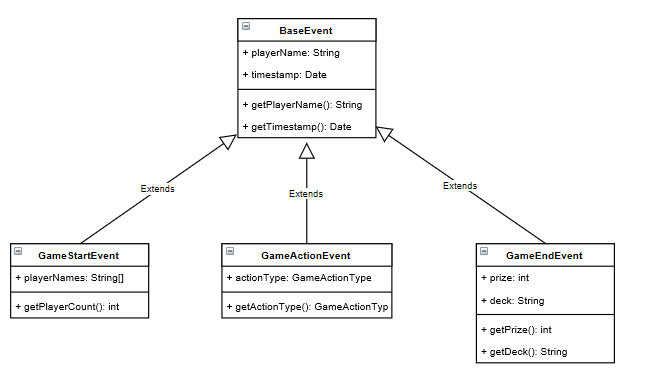
\includegraphics[width=\textwidth,height=\textheight,keepaspectratio]{images/Events.png}
	\caption{Event Klassen des Szenarios}
	\label{EventKlassen}
\end{figure}

Um das Szenario abzubilden werden verschiedene Event-Klassen benötigt. Mit diesem Begriff sind Klassen gemeint, die ein Event darstellen.
Als gemeinsame Basis dient die Event-Klasse \textbf{BaseEvent} (Siehe Abbildung \ref{EventKlassen}). Dieses Event beinhaltet den Spieler-Namen und einen Zeitstempel. Diese beiden Felder werden in allen Events benötigt.

Die Event-Klassen \textbf{GameStartEvent} und \textbf{GameEndEvent} bilden den Start und das Ende einer Poker-Partie ab. Zu Beginn (\textbf{GameStartEvent}) werden alle Spiel-Teilnehmer benötigt, gegen Ende (\textbf{GameEndEvent}) das Preisgeld und Kartendeck, welches gewonnen hat. Da beide Events von \textbf{BaseEvent} erben, besitzen sie automatisch einen Zeitstempel und den zugeordneten Spieler. Beim Spielstart wird der Name des ersten Spielers verwendet.

Im Laufe der Partie werden verschiedene Aktionen der Spieler durchgeführt. Diese sind durch die Event-Klasse \textbf{GameActionEvent} abgebildet. Das Event beinhaltet ein Feld für die Aktionsart (z.B. "rise", wenn ein Spieler erhöht hat).

\subsection{Architektur}
\label{kapitel_architektur}
Die nachfolgende Abbildung zeigt die Architektur von Esper. Dabei ist sie, auf die in der Umsetzung benötigten Komponenten, beschränkt.

\begin{figure}[ht]
	\centering
	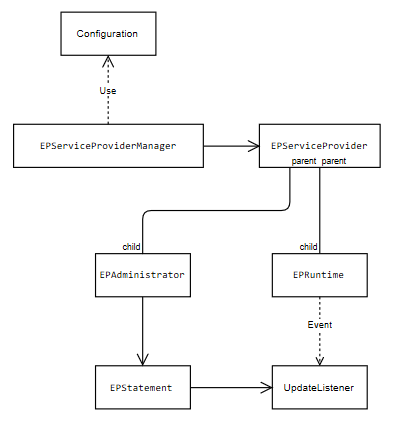
\includegraphics{images/Architektur.png}
	\caption{Architektur von Esper}
	\label{architektur}
\end{figure}

Die \textbf{Configuration}-Klasse wird verwendet, um die Esper-Engine zu konfigurieren. Unter anderem lassen sich dort die Event-Typen registrieren, die verarbeitet werden sollen. Neben den Event-Typen, gibt es die Möglichkeit Plugins zu registrieren. 

Durch Plugins werden benutzerdefinierte Funktionen eingebunden (z.B für den Vergleich von Geo-Koordinaten).
Nachfolgend zeigt die Basis-Konfiguration der Umsetzung:

\begin{lstlisting}[caption={Basis-Konfiguration}\label{lst:basisKonfiguration},captionpos=t,language=JAVA]

import com.espertech.esper.client.Configuration
import de.htwg.da.esper.sample.event.GameActionEvent;
import de.htwg.da.esper.sample.event.GameEndEvent;
import de.htwg.da.esper.sample.event.GameStartEvent;

Configuration config = new Configuration();

// Register event types to observe
config.addEventType("GameStart",GameStartEvent.class.getName());
config.addEventType("Action", GameActionEvent.class.getName());
config.addEventType("GameEnd", GameEndEvent.class.getName());
\end{lstlisting}

In der Konfiguration werden die Event-Typen \textbf{GameStartEvent}, \textbf{GameActionEvent} und \textbf{GameEndEvent} registriert. Plugins werden nicht verwendet.

Über die \textbf{EPServiceProviderManager}-Klasse kann der \textbf{EPServiceProvider} erhalten werden:

\begin{lstlisting}[caption={EPServiceProvider}\label{lst:epServiceProvider},captionpos=t,language=JAVA]

import com.espertech.esper.client.*;

EPServiceProvider cep = EPServiceProviderManager.
getProvider("MyEsperProvider", config);
\end{lstlisting}


Der erste Parameter stellt eine eindeutige Bezeichnung für den Provider dar. Dadurch ist es möglich, mehrere \textbf{EPServiceProvider} und damit mehr als eine Esper-Engine parallel zu verwenden. Als zweiter Parameter wird die zuvor  erstellte Konfiguration (siehe Quelltext \ref{lst:basisKonfiguration}) verwendet.

Der \textbf{EPServiceProvider} hält die Referenzen auf die Klassen \textbf{EPAdministrator} und \textbf{EPRuntime}. 

\subsection{Events versenden}
Für das Versenden eines Events wird die Methode \textbf{sendEvent(...)} der Klasse \textbf{EPRuntime} verwendet (siehe Abbildung \ref{architektur}). Als Parameter kann eine beliebige Event-Klasse übergeben werden, wie nachfolgend mit einem \textbf{GameStartEvent} dargestellt:

\begin{lstlisting}[caption={Event versenden}\label{lst:fireEvent},captionpos=t,language=Java]

EPServiceProvider cep = EPServiceProviderManager.
			getProvider("MyEsperProvider",esperConfig);

final EPRuntime cepRT = cep.getEPRuntime();

// Fire sample event
cepRT.sendEvent(new GameStartEvent());
\end{lstlisting}

\subsection{Events generieren}
Damit die Events für das Szenario einfach erzeugt und versendet werden können, wird eine Hilfs-Klasse (\textbf{EventGenerator}) verwendet. Dieser ist zuständig für die Generierung von Beispiel-Events (z.B. \textbf{GameActionEvent}).

\begin{lstlisting}[caption={Event Generator}\label{eventGenerator},captionpos=t,language=Java]
public final class EventGenerator {
  private static String[] PLAYER_NAMES = {"Clemens", "Lukas", "Kathrin"};
  private static Random GENERATOR = new Random();
  
  public static GameActionEvent randomGameActionEvent() {
    final String playerName = randomPlayerName();
    final Date timestamp = randomTimestamp();
    final GameActionType gameActionType = randomGameActionType();
    return new GameActionEvent(playerName, timestamp, gameActionType);
  }

  private static GameActionType randomGameActionType() {
    int gameActionTypeIndex = GENERATOR.nextInt(GameActionType.values().length);
    return GameActionType.values()[gameActionTypeIndex];
  }

  private static String randomPlayerName() {
    int playerIndex = GENERATOR.nextInt(PLAYER_NAMES.length);
    String playerName = PLAYER_NAMES[playerIndex];
    return playerName;
  }

  private static Date randomTimestamp() {
    long timeStamp = System.currentTimeMillis();
    return new Date(timeStamp);
  }
}
\end{lstlisting}

Zur besseren Übersichtlichkeit sind nicht alle Methoden im Quellcode \ref{eventGenerator} enthalten.
Gezeigt wird, dass über den Aufruf der Methode \textbf{randomGameActionEvent()} ein zufälliges \textbf{GameActionEvent} erzeugt wird. Hierzu werden für das zu erzeugende Event ein zufälliger Spieler-Name, Zeitstempel und Aktionstyp generiert. Die möglichen Werte können konfiguriert werden. Im obigen Beispiel sind dies ''Clemens'', ''Lukas'' und ''Kathrin'' als Spieler-Namen, die aktuelle Zeit als Zeitstempel und ein zufälliger Aktionstyp aus den möglichen Aktionen in Poker.

\subsection{Events verarbeiten}
\label{EventsVerarbeiten}
Für das Verarbeiten von Events wird ein Statement (siehe Kapitel \ref{statements}) benötigt, um die gewünschten auszuwählen und ein UpdateListener, um es anschließend zu verarbeiten. Dieser spezielle Listener ist in der Esper-Bibliothek enthalten und enthält nur eine einzige Methode. Nachfolgend zeigt eine beispielhafte Implementierung für das Szenario der Ausarbeitung:

\begin{lstlisting}[caption={UpdateListener}\label{updateListener},captionpos=t,language=Java]
public class GameActionListener implements UpdateListener {

public void update(EventBean[] newData, EventBean[] oldData) {
Object event = newData[0].getUnderlying();

System.out.println("------> Game action: " + event);
}
}
\end{lstlisting}

Der \textbf{UpdateListener}, in der Abbildung GameActionListener genannt, erhält in der Methode \textbf{update(EventBean[] newData, EventBean[] oldData)} die aktuellen Events als ersten und die vorherigen als zweiten Parameter. Dadurch ist es möglich auf Beziehung zwischen Events zu schließen (Kausalität).

Anschließend wird über eine \textbf{System out}-Anweisung die aktuelle Aktion ausgegeben. Sind mehr als 1 Event im ersten Parameter der Methode enthalten, wird nur das erste ausgewertet (Das neuste Element). Die anderen Elemente wurden bereits zuvor abgearbeitet, da der \textbf{UpdateListener}, in diesem Beispiel, auf ein Statement hört, welches ein Length-Window (siehe \ref{LengthWindow}) verwendet, dies ist in der Abbildung nicht dargestellt.

Dies bedeutet auch, dass sich die Logik innerhalb des \textbf{UpdateListener} immer auch auf das gegebene Statement beziehen sollte. Wird z.B. ein Length-Batch-window (siehe \ref{LengthBatchWindow}) verwendet, müssen alle Events verarbeitet werden, wenn der \textbf{UpdateListener} aufgerufen wird, da dies erst geschieht, wenn das Window genau so viele Events wie angegeben enthält. Bei einem Length-Window (siehe \ref{LengthWindow}) muss immer nur das Neuste verarbeitet werden, weil dort der \textbf{UpdateListener} bei jedem Event ausgelöst wird. 

Dies zeigt auch, wie Komplex in Esper die Steuerung der Weiterverarbeitung von Events werden kann. 